\documentclass[12pt]{extreport}

\usepackage{lipsum}
\usepackage{extsizes}
\usepackage{graphicx}
\graphicspath{{./images/}}
\usepackage{caption}
\usepackage{listings}
\usepackage{wrapfig}
\usepackage{blindtext}
\usepackage{xcolor}

\usepackage{courier}
\usepackage{color}

\definecolor{mygreen}{rgb}{0,0.6,0}
\definecolor{mygray}{rgb}{0.5,0.5,0.5}
\definecolor{mymauve}{rgb}{0.58,0,0.82}
\lstset{ %
    backgroundcolor=\color{white},   % choose the background color; you must add \usepackage{color} or \usepackage{xcolor}
    basicstyle=\footnotesize\ttfamily,        % the size of the fonts that are used for the code
    breakatwhitespace=false,         % sets if automatic breaks should only happen at whitespace
    breaklines=true,                 % sets automatic line breaking
    captionpos=b,                    % sets the caption-position to bottom
    commentstyle=\color{mygreen},    % comment style
    deletekeywords={...},            % if you want to delete keywords from the given language
    escapeinside={\%*}{*)},          % if you want to add LaTeX within your code
extendedchars=true,              % lets you use non-ASCII characters; for 8-bits encodings only, does not work with UTF-8
frame=single,                    % adds a frame around the code
keepspaces=true,                 % keeps spaces in text, useful for keeping indentation of code (possibly needs columns=flexible)
keywordstyle=\color{blue},       % keyword style
otherkeywords={*,...},            % if you want to add more keywords to the set
numbers=left,                    % where to put the line-numbers; possible values are (none, left, right)
numbersep=5pt,                   % how far the line-numbers are from the code
numberstyle=\tiny\color{mygray}, % the style that is used for the line-numbers
rulecolor=\color{black},         % if not set, the frame-color may be changed on line-breaks within not-black text (e.g. comments (green here))
showspaces=false,                % show spaces everywhere adding particular underscores; it overrides 'showstringspaces'
showstringspaces=false,          % underline spaces within strings only
showtabs=false,                  % show tabs within strings adding particular underscores
stepnumber=2,                    % the step between two line-numbers. If it's 1, each line will be numbered
stringstyle=\color{mymauve},     % string literal style
tabsize=2,                       % sets default tabsize to 2 spaces % show the filename of files included with \lstinputlisting; also try caption instead of title,
}

\renewcommand{\lstlistingname}{\bfseries Popis}

\captionsetup[figure]{justification=raggedright, singlelinecheck=false, labelfont={bf}, textfont={Noto Mono}}

%! Author = Karlo
%! Date = 23.9.2023.

% Preamble
\documentclass[11pt]{article}

% Packages
\usepackage{amsmath}

% Document
\begin{document}



\end{document}
%From M275 "Topology" at SJSU
\newcommand{\id}{\mathrm{id}}
\newcommand{\taking}[1]{\xrightarrow{#1}}
\newcommand{\inv}{^{-1}}

%From M170 "Introduction to Graph Theory" at SJSU
\DeclareMathOperator{\diam}{diam}
\DeclareMathOperator{\ord}{ord}
\newcommand{\defeq}{\overset{\mathrm{def}}{=}}

%From the USAMO .tex files
\newcommand{\ts}{\textsuperscript}
\newcommand{\dg}{^\circ}
\newcommand{\ii}{\item}

% % From Math 55 and Math 145 at Harvard
% \newenvironment{subproof}[1][Proof]{%
% \begin{proof}[#1] \renewcommand{\qedsymbol}{$\blacksquare$}}%
% {\end{proof}}

\newcommand{\liff}{\leftrightarrow}
\newcommand{\lthen}{\rightarrow}
\newcommand{\opname}{\operatorname}
\newcommand{\surjto}{\twoheadrightarrow}
\newcommand{\injto}{\hookrightarrow}
\newcommand{\On}{\mathrm{On}} % ordinals
\DeclareMathOperator{\img}{im} % Image
\DeclareMathOperator{\Img}{Im} % Image
\DeclareMathOperator{\coker}{coker} % Cokernel
\DeclareMathOperator{\Coker}{Coker} % Cokernel
\DeclareMathOperator{\Ker}{Ker} % Kernel
\DeclareMathOperator{\rank}{rank}
\DeclareMathOperator{\Spec}{Spec} % spectrum
\DeclareMathOperator{\Tr}{Tr} % trace
\DeclareMathOperator{\pr}{pr} % projection
\DeclareMathOperator{\ext}{ext} % extension
\DeclareMathOperator{\pred}{pred} % predecessor
\DeclareMathOperator{\dom}{dom} % domain
\DeclareMathOperator{\ran}{ran} % range
\DeclareMathOperator{\Hom}{Hom} % homomorphism
\DeclareMathOperator{\Mor}{Mor} % morphisms
\DeclareMathOperator{\End}{End} % endomorphism

\newcommand{\eps}{\epsilon}
\newcommand{\veps}{\varepsilon}
\newcommand{\ol}{\overline}
\newcommand{\ul}{\underline}
\newcommand{\wt}{\widetilde}
\newcommand{\wh}{\widehat}
\newcommand{\vocab}[1]{\textbf{\color{blue} #1}}
\providecommand{\half}{\frac{1}{2}}
\newcommand{\dang}{\measuredangle} %% Directed angle
\newcommand{\ray}[1]{\overrightarrow{#1}}
\newcommand{\seg}[1]{\overline{#1}}
\newcommand{\arc}[1]{\wideparen{#1}}
\DeclareMathOperator{\cis}{cis}
\DeclareMathOperator*{\lcm}{lcm}
\DeclareMathOperator*{\argmin}{arg min}
\DeclareMathOperator*{\argmax}{arg max}
\newcommand{\cycsum}{\sum_{\mathrm{cyc}}}
\newcommand{\symsum}{\sum_{\mathrm{sym}}}
\newcommand{\cycprod}{\prod_{\mathrm{cyc}}}
\newcommand{\symprod}{\prod_{\mathrm{sym}}}
\newcommand{\Qed}{\begin{flushright}\qed\end{flushright}}
\newcommand{\parinn}{\setlength{\parindent}{1cm}}
\newcommand{\parinf}{\setlength{\parindent}{0cm}}
% \newcommand{\norm}{\|\cdot\|}
\newcommand{\inorm}{\norm_{\infty}}
\newcommand{\opensets}{\{V_{\alpha}\}_{\alpha\in I}}
\newcommand{\oset}{V_{\alpha}}
\newcommand{\opset}[1]{V_{\alpha_{#1}}}
\newcommand{\lub}{\text{lub}}
\newcommand{\del}[2]{\frac{\partial #1}{\partial #2}}
\newcommand{\Del}[3]{\frac{\partial^{#1} #2}{\partial^{#1} #3}}
\newcommand{\deld}[2]{\dfrac{\partial #1}{\partial #2}}
\newcommand{\Deld}[3]{\dfrac{\partial^{#1} #2}{\partial^{#1} #3}}
\newcommand{\lm}{\lambda}
\newcommand{\uin}{\mathbin{\rotatebox[origin=c]{90}{$\in$}}}
\newcommand{\usubset}{\mathbin{\rotatebox[origin=c]{90}{$\subset$}}}
\newcommand{\lt}{\left}
\newcommand{\rt}{\right}
\newcommand{\bs}[1]{\boldsymbol{#1}}
\newcommand{\exs}{\exists}
\newcommand{\st}{\strut}
\newcommand{\dps}[1]{\displaystyle{#1}}

\newcommand{\sol}{\setlength{\parindent}{0cm}\textbf{\textit{Solution:}}\setlength{\parindent}{1cm} }
\newcommand{\solve}[1]{\setlength{\parindent}{0cm}\textbf{\textit{Solution: }}\setlength{\parindent}{1cm}#1 \Qed}
%! Author = Karlo
%! Date = 23.9.2023.

% Preamble
\documentclass[11pt]{article}

% Packages
\usepackage{amsmath}

% Document
\begin{document}



\end{document}

\title{\Huge{Osnove web programiranja}}
\author{\huge{Karlo Vizec}}
\date{\today}

\begin{document}

    \maketitle
    \newpage% or \cleardoublepage
% \pdfbookmark[<level>]{<title>}{<dest>}
    \pdfbookmark[section]{\contentsname}{toc}
    \tableofcontents
    \pagebreak

    \chapter*{Predgovor}\label{ch:predgovor}

Računala prošlosti bila su ogromna.
Tijekom sredine prošlog stoljeća zauzimala su cijele prostorije, a bila sporija od najslabijeg suvremenog mobitela.
Imala su vrlo malu memoriju te je njihova funkcija bila ograničena procesorskom snagom koja je bila niska.
Međutim, najbitnija činjenica za nas je da nisu bila povezana.

Recimo da želite instalirati Windows 3.0 na vaše novo IBM osobno računalo tijekom 1990.
Vaš prvi korak je da odete do najbližeg dućana s računalima i kupite fizički primjerak Windowsa na disketi.
Kada stignete doma, tu disketu bi ubacili u vaše računalo i instalirali Windows.
Tada Internet nije postojao, niste mogli samo otvoriti microsoft.com i preuzeti najnoviju verziju.
Muzika se prenosila pomoću disketa, i kasnije CD-a i DVD-a, a videi su bili vrlo rijetki na računalima.

Danas je Internet jedan od najvažnijih dijelova našeg života, postao je novi način na koji prikupljamo informacije i razmišljamo.
Jedna rečenica objavljena na Twitteru od strane neke poznate osobe može imati ogroman utjecaj.
Zbog toga računala i mobiteli postaju sve više samo platforme za web preglednike.
Razne tvrtke to primjećuju i prilagođavaju svoji model poslovanja.
Nove tehnologije omogućuje da sve više i više aplikacija i programa postanu web stranice (web aplikacije) bez potrebe preuzimanja.

Programeri nisu slijepi na te promjene, a to se lako može primijetiti u činjenici da su jezici za web programiranje, načelno HTML, CSS i JavaScript, među najpopularnijim.
Štoviše, prema 2023.\ anketi za programere StackOverflowa, JavaScript je \textit{najpopularniji} programski jezik, a drugi najpopularniji su HTML i CSS.

Ovaj udžbenik sam napisao s ciljem otvaranja svijet informatike i programiranja srednjoškolcima i naprednim osnovnoškolcima.
Namijenjen je primarno za fakultativnu nastavu i/ili izvannastavne aktivnosti iz informatike i programiranja.
U udžbeniku ima dovoljno materijala za ~35 školskih sati godišnje, ovisno o opsežnosti nastave.
Nadam se da će ovaj udžbenik pridonijeti smanjivanju praga za učenje programiranja učenicima.

\medskip
\begin {flushright}
    \textit{Karlo Vizec, listopad 2023.}
\end {flushright}


    \chapter{Uvod u web programiranje}\label{ch:uvod-u-web-programiranje}

\section{Internet ukratko}\label{sec:internet-ukratko}

\subsection{Računalne mreže}\label{subsec:racunalne-mreze}

Internet kao koncept najlakše se može zamisliti kao \("\)mreža od mreža\("\).
Računalne mreže postoje kako bi omogućile međusobno povezivanje računala i drugih uređaja u svrhe međusobne komunikacije.

Te računalne mreže od kojih se sastoji Internet uključuju one najmanje, \textbf{LAN} (engl. \textit{Local Area Network}) mreže koje se nalaze u kućama i stanovima svih ljudi.
One se obično sastoje od rutera, nekoliko računala i mobitela, televizora te još neke opreme.
Sljedeća najbitnija razina mreže je \textbf{WAN} (engl. \textit{Wide Area Network}).
Točan opseg WAN mreže nije strogo definiran te može zahvaćati područje od veličine neke velike škole ili sveučilišta pa sve do cijele države.
Glavna razlika između WAN i LAN mreža je u geografskom području koje zauzimaju.
WAN mreže će obično imati naprednije sustave koji su potrebni za upravljanje tako velikim prostorom.

Još kategorija računalnih mreža postoje, uključujući \textbf{Personal Area Network (PAN)} i \textbf{Metropolitan Area Network (MAN)}.
PAN mreže su nekoliko metara u veličini.
Primjer takve mreže su mobitel i slušalice spojene pomoću WiFi-a ili Bluetootha.
MAN mreže obično su one mreže koje povezuju veće područje, recimo neki grad ili naselje.

Pristup Internetu daju pružatelji internetskih usluga (engl. \textit{Internet Service Provider}, \textbf{ISP}).
Za veliku većinu osoba, taj pristup biti će u obliku uređaja koji se zove \textbf{ruter} (od engl. \textit{router}).
Ruter je uređaj koji služi kao glavna pristupna točka Internetu, na njega se, žično ili bežično, povezuju drugi uređaji koji zahtjevaju pristup Internetu, ali i ostalim uređajima u LAN mreži.
Njegova svrha je komunikacija između uređaja u njegovoj mreži i šireg Interneta.
On odašilje i prima (te onda šalje uređaju koji je namijenjeni primatelj) pakete podataka koje šalju i primaju uređaji povezani u mrežu putem rutera.

\begin{figure}[h]\label{fig:lan-diagram}
    \centering
    \vspace*{-3cm}
    
\includegraphics[scale=0.125]{lan-diagram}
    \vspace*{-3cm}
    \caption{Dijagram jednostavne LAN mreže s ruterom i nekoliko uređaja povezanih na njega. Kompliciranije LAN mreže mogu imati i mrežni preklopnik (engl. \textit{switch}). Izvor: Cloudflare.}
\end{figure}

Komponente mreže prikazane na Slici 1.1 jesu one najčešće.
Međutim, postoje i druge komponente mreža.
Ruter, recimo, nije nužan da bi se stvorila mreža.
Primjer uređaja koji može zamjeniti neke svrhe rutera je \textbf{mrežni preklopnik}.
On povezuje računala u mrežu u obliku zvijezde tako što koordinira slanje poruka između računala i omogućava im da komuniciraju međusobno.
Glavna razlika između preklopnika i rutera je ta što preklopnik ne može sam povezati svoju mrežu s vanjskim svijetom Interneta.
Međutim, preklopnici su često spojeni na ruter te tako mogu povezati računala s ostatkom Interneta.

\begin{figure}[h]\label{fig:switch-lan-diagram}
    
\includegraphics[scale=0.3375,left]{switch-diagram}
    \raggedleft
    \caption{Dijagram LAN mreže s mrežnim preklopnikom. Izvor: Cloudflare.}
\end{figure}

\newpage
\subsection{Arhitektura}\label{subsec:arhitektura}

Internet je, dakle, ogromna računalna mreža koja se sastoji od milijardi računalna, od pametnih telefona do ogromnih, specijaliziranih servera.
Internetovi korijeni sežu do sredine 20.\ stoljeća kada je američka agencija ARPA\footnote{ARPA, odnosno DARPA, je nekoliko puta promjenila ime iz Advanced Research Projects Agency (ARPA) u Defense Advanced Research Projects Agency (DARPA) tijekom zadnjih nekoliko desetljeća da bi stala na trenutnom DARPA nazivu.} radila na skupu projekata sponzoriranih od strane američke vlade.
Nekakva prva inkarnacija Interneta bio je \textbf{ARPANET}, razvijen 1969.
Većinom je povezivao sveučilišta.
Tijekom godina projekt izrade Interneta prešao je iz Vladinih u akademske i istraživačke ruke da bi u suvremenom dobu postao uglavnom komercijalni, međunarodni projekt.

Jezgra Interneta sastoji se od nekoliko ogromnih, međunarodnih korporacija (ISP-ova) koji su vlasnici nekoliko skupina međusobno povezanih mreža s velikim protokom.
Glavni dio tih mreža je skupina podvodnih komunikacijskih kablova koji povezuju Internet između kontinenata.
\begin{figure}[h]
    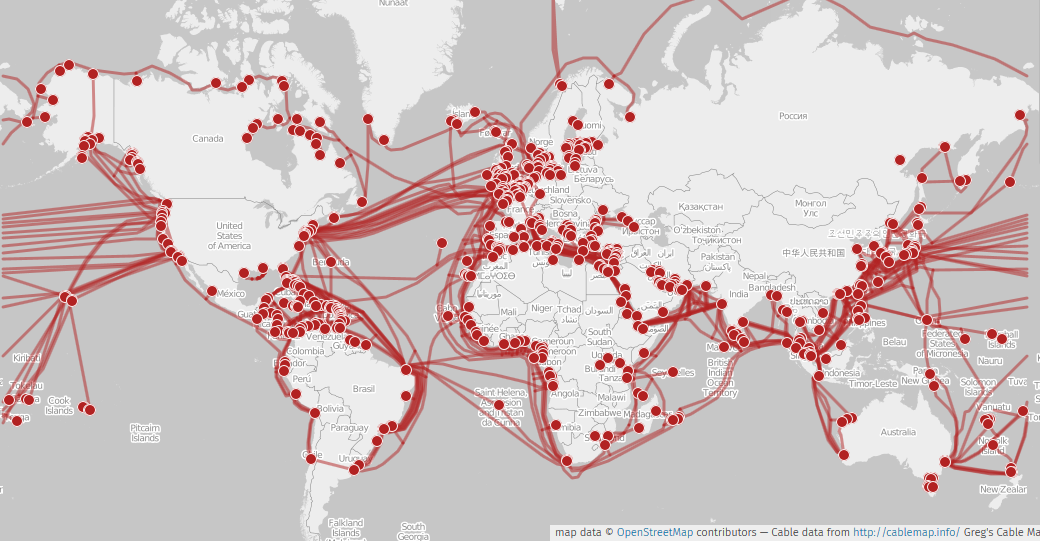
\includegraphics[scale = 0.48]{internet-underwater-backbone}
    \caption{Međukontinentalna mreža podvodnih komunikacijskih kablova koji služe kao kralježnica Interneta iz 2015. Izvor: OpenStreetMap. }\label{fig:figure6}
\end{figure}
Zbog činjenice da je Internet toliko rasprostranjen i dobro povezan, vrlo je niska vjerojatnost da, čak i ako neki dio Interneta prestane raditi, će cijeli sustav pasti.

\mlenma{Kako ugasiti Internet?}{
    \sffamily
    Možda ste čuli s vremena na vrijeme da neka hakerska skupina prijeti da će ugasiti Internet ili da neka organizacija ili osoba može ugasiti Internet.
    Iz ovoga što ste naučili do sada, jasno je da je to nemoguće.
    Internet nije neki centralizirani sustav koji ima tipku za gašenje.
    Internet je potpuno obrnuto od toga.
    Najviše što jedna organizacija može učiniti je otežati rad Interneta, ali ga ne može onesposobiti u potpunosti.
}

Bilo koji sustav s milijardi uređaja povezanih na njega s mogućnosti međusobne komunikacije između uređaja zahtjeva mehanizam za adresiranje uređaja.
Odnosno, način da se odredi tko je tko.
Na Internetu taj su mehanizam \textbf{IP (Internet Protocol) adrese}.
IP adrese su brojevi.
Najčešći oblik IP adrese koji ste vidjeli i onaj koji je prvi bio napravljen su \textbf{IPv4 adrese}\footnote{IPv4 označuje četvrtu verziju Internet Protokola.}.
IPv4 adrese sastoje se od 32 bita, što znači da je maksimalni broj IPv4 adresa $ 2^{32} $ (4,294,967,796).
Drugim riječima, najveći broj uređaja koji mogu biti adresirani na Internetu pomoću IPv4 adresa je $ 2^{32} $.

IPv4 adrese se zapisuju u obliku četiri 8-bitnih brojeva odjeljeni s točkom: \verb|A.B.C.D|.
Primjeri IPv4 adresa uključuju \verb|8.8.8.8|, \verb|245.40.3.36| i \verb|123.123.123.123|.
Najveći osmobitni broj je $ 2^8 - 1 $ (255).
Dakle, svaki broj u IPv4 adresi ne može biti veći od 255, odnosno najveća IPv4 adresa je \verb|255.255.255.255|.

U početku je to bilo više nego dovoljno.
Nitko nije mogao predvidjeti da će Internet postati ovakva grdosija kakva je danas.
Polako je to postalo nedovoljno jer se sve više računala povezivalo na Internet.
IPv4 adrese postaju sve skuplje zbog toga (velika potražnja, mala ponuda).
Internet je danas u procesu prebacivanja na \textbf{IPv6 adrese} koje se sastoje od 128 bitova.
Dakle, s IPv6 adresama, je moguće adresirati $ 2^{128} $ uređaja na Internetu.
IPv6 adrese se zapisuju u obliku osam četveroznamenkastih heksadekadskih brojeva odvojeni s dvotočkom.

Možda ste primjetili da kada otvarate neku stranicu, većinom ne upisujete IP adresu njezinog servera iako je to ono što vaš preglednik u konačnici koristi da ju otvori.
Ako ju uopće izravno otvarate, obično upisujete njezinu \textbf{domenu}, npr. \verb|youtube.com|.
Domena je naziv (string) koji označava određenu web stranicu ili područje unutar Interneta.
Postoji nekoliko vrsta domena.
Najviša razina su \textbf{vršne domene} (engl. \textit{top-level domains}, \textbf{TLDs}).
One uključuju \verb|.com|, \verb|.net|, \verb|.org|, \verb|.edu|, \verb|.hr|.

Vršne domene se mogu nadalje podjeliti na \textbf{generičke domene} (\textbf{gTLDs}, npr. \verb|.com|, \verb|.edu|, \verb|.net|, itd.) i \textbf{geografske domene} (\textbf{ccTLDs}, npr. \verb|.hr|, \verb|.us|, \verb|.uk|, \verb|.de|, itd.).
Generičke domene sastoje se od tri znaka, a geografske od dva.

Pomoću vršnih domena mogu se registrairati vlastite domene preko \textbf{registara domena}.
Gotovo svaka stranica na Webu ima svoju domenu.
Domene nisu ni skupe za registrirati.
Prosječna \verb|.com| ili \verb|.net| domena košta oko 10€ godišnje.
Uz domene je moguće registrirati i beskonačni broj \textbf{poddomena}, npr. \verb|ocjene.skole.hr| ili \verb|www.google.com|.
Organizacija koja je zadužena za upravljanjem domena je Internetska koporacija za dodjeljena imena i brojeve (engl. \textit{Internet Corporation for Assigned Names and Numbers}, \textbf{ICANN}).

\mlenma{Kako je poddomena \texttt{www} došla svuda}{
    \sffamily
    Vjerojatno ste primjetili da su domene mnogo stranica \texttt{www.example.com} umjesto \texttt{example.com}.
    Razlog za ovo je povijesni.
    Već znate da je WWW, Web, povezan sa, ali odvojen od Interneta.
    Kada je Web bio napravljen, bio je samo još jedan dio Interneta, a ne glavni kao što je sada, pa je dobio svoju poddomenu, \texttt{www}.
    Kako je Web postajao sve popularniji, sve je više web stranica bilo napravljeno i one su pratile tradiciju da im glavna stranica bude na poddomeni \texttt{www}.
    Međutim, tijekom zadnjih nekoliko godina, ta je tradicija sve manje popularna.
}

Međutim, domene služe isključivo kako bi olakšale korisnicima da pronađu stranice, samo adresiranje računala na Internetu (pa tako i servera na kojim se nalaze web stranice) još uvijek se odvija pomoću IP adresa.
Kada vi upišete domenu neke stranice, vaš preglednik mora saznati IP adresu servera te stranice.
To se događa pomoću \textbf{DNS-a} (engl. \textit{Domain Name System}).
DNS sustav je hijerarhiski.
To znači da vaše računalo ne mora imati lokalnu kopiju cijelog DNS-a.
Umjesto toga, vaše računalo samo mora znati pronaći najbliži DNS server, obično onaj od vašeg ISP-a.
Serveri koji na sebi sadrže informacije o povezanosti raznih domena s IP adresama i pomažu pri konverziji nazivaju se \textbf{imenski serveri}.

Taj DNS server također ne mora imati cijeli DNS pohranjen na sebe.
Potraga za pravom IP adresom stranice započinje od vršne domene stranice sve do konačnog imenskog servera koji će odgovoriti s točnom IP adresom stranice.

\subsection{Protokoli i WWW}\label{subsec:protokoli-i-www}

Internet funkcionira zbog raznih \textbf{protokola}.
U kontekstu Interneta, protokol je skupina definiranih, standardiziranih pravila koja određuju kako će dva ili više računala surađivati.
Postoje stotine protokola koji se koriste na Internetu.
Glavna skupina od nekoliko desetaka nazivaju se grupnim imenom \textbf{TCP/IP} prema dva glavna protokola: TCP (engl. \textit{Transmission Control Protocol}) i IP (engl. \textit{Internet Protocol}).

Na elementarnoj razini, Internet je zapravo samo mehanizam pomoću kojeg računala razmjenjuju poruke.
Te se poruke ne šalju sve odjednom nego u \textbf{paketima}.
Paketi su djelovi poruka pomoću kojih se poruke na Internetu razmjenjuju i onda sastave u jednu cjelinu na odredištu.
TCP je protokol koji koordinira razmjenu poruka između računala.
Postoje i alternative TCP-u, npr. \textbf{UDP} (engl. \textit{User Datagram Protocol}).
UDP se često koristi za \textit{streamanje} videa preko mreže jer, za razliku od TCP-a, UDP ne zahtjeva da svi paketi uspješno stignu na odredištu.
Kada gledate video, puno je prihvatljivije da iskusite kratak pad u kvaliteti ili trzaj jer neki paket nije stigao nego da video zastane na par sekundi dok server ne pošalje ponovno taj paket.

Uz te protokole, postoje i mnogi drugi.
\textbf{SMTP} (engl. \textit{Simple Mail Transfer Protocol}) se koristi za slanje i primanje emailova.
\textbf{FTP} (engl. \textit{File Transfer Protocol}) služi za razmjenu datoteka između korisnika i servera.

\textbf{World Wide Web (WWW)} započeo je s CERN-ovim znanstvenikom Tim Berners-Lee.
CERN je europska organizacija u kojoj znanstvenici rade na sudaranju sitnih čestica s još manjim česticama u nadi da će tako otkriti od čega je napravljen svemir.
Njega je navodno manje zanimalo uništavanje Zemlja pa je odlučio pokušati napraviti Web.
Web je bio baziran na ideji \textbf{hiperveza}, poveznice koje međusobno vežu dokumente.
Taj se koncept nama danas čini primitivnim, ali je tada bio revolucionaran.

Na Webu postoje dva glavna aktera: \textbf{klijenti} (korisnici, web preglednici, itd.) i \textbf{serveri}.
Server je računalni program koji prima, obrađuje i odgovara na zahtjeve klijenata.
\textbf{Čvor} je fizičko računalno na kojem se nalaze jedan ili više servera.
Klijent je računalni program koji šalje i prima odgovore na zahtjeve serveru.
Jedan program može, i često je, klijent i server.
Serveri često moraju pristupiti nekoj vrsti baze podataka, koja je ujedno i server.

\begin{figure}[h]
    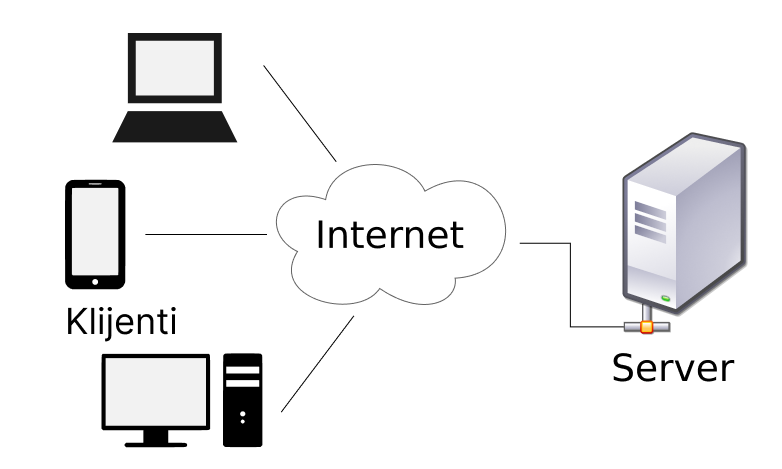
\includegraphics[scale=0.3]{client-server-model}
    \caption{Model klijenta i servera. Izvor: Wikipedija.}\label{fig:figure7}
\end{figure}

Komunikaciju između klijenta i servera na Webu obično diktira \textbf{HTTP} (engl. \textit{HyperText Transfer Protocol}).
HTTP sam po sebi nije siguran pa je zato kasnije razvijen \textbf{HTTPS} (engl. \textit{HyperText Transfer Protocol Secure}).
HTTPS je prvotno koristio \textbf{SSL} protokol (engl. \textit{Secure Sockets Layer}).
Međutim, danas se više ne koristi SSL nego \textbf{TLS} (engl. \textit{Transport Layer Security}).
Ti protokoli osiguravaju da će poruke poslane između klijenta i servera biti vidljive samo njima dvoje.
To čini koristeći enkripciju.

Tri ključna jezika Weba su HTML, CSS i JavaScript.
Prvo je postojao samo HTML.\@
Nakon nekog vremena, programerima je dosadilo gledati statični tekst koji izgleda vrlo ružno.
Pa je onda napravljen JavaScript, prvotno namjenjen kao jednostavni skriptni jezik koji bi omogućio programerima da dodaju neku razinu interaktivnosti stranicama.
Danas se JavaScript koristi za razne primjene daleko van onih zamišljenih kada ga je Brendan Eich napravio u 10 dana 1995.
Sljedeći dodatak Webu bio je CSS 1996.
CSS dopušta promjenu izgleda elementima na web stranicama.

\mlenma{Linux: Operacijski sustav koji pokreće Web}{
    \sffamily
    Najpopularniji operacijski sustav za kućnu upotrebu na PC-ovima je Windows.
    Vi ga vjerojatno koristite na svojem računalu.
    Međutim, vrlo mali udio servera koji čine Web koriste Windows.
    Iako postoji inačica Windowsa za servere, kreativno nazvana Windows Server, čak i sam Microsoft koristi alternativu.

    Ta je alternativa Linux, napravio ga je Linus Torvalds 1991., švedski programer po kojem je taj operacijski sustav i nazvan.
    Zbog činjenice da je Linux besplatan te njegov kod javno dostupan vrlo je primamljiv za programere i administratore servera.
    Raznorazni alati ključni za održavanje servera rade samo na Linuxu te zato i mnogo programera koristi Linux na svojim osobnim računalima.
    Čak ga i sam Microsoft koristi.
    Glavna mana za korištenje Linuxa na osobnim računalima je manjak programske podrške za njega (npr., programi Adobea ne podržavaju Linux), ali i ta se situacija krenula poboljšavati.

    Linux sam po sebi nije potpuni operacijski sustav već najbitniji dio koji se naziva \textbf{kernel}.
    Kernel je najosnovniji i ključni dio operacijskog sustava koji upravlja sklopovljem računala i osnovnim funkcijama.
    Cielokupni Linux paketi koji sadrže sve potrebno za upotrebu (grafičko sučelje, razne programe i ostale osnovne, upravljačke programe) nazivaju se \textbf{Linux distribucije}.
    Među najpopularnijim distribucijama (ili \textit{distroima} kako ih često zovu) jesu Debian, Fedora i Arch Linux.
    Ostatak popularnih distroa su bazirani na ova tri, uključujući i Ubuntu čija je baza Debian.
    Zbog Linuxove licencije, sve njegove distribucije su besplatne kao i on.
}

\section{Postavljanje radnog okruženja}\label{sec:postavljanje-radnog-okruzenja}

U školi ste vjerojatno uglavnom programirali u Pythonu te za to koristili njegovog radnog orkuženje, IDLE.
Python je jedan od rijetkih programksih jezika koji imaju svoje službeno radno orkuženje.
IDLE je koristan za učenje Pythona, ali je u osnovi Blok za pisanja s mogućnosti pokretanja napisanih programa.
Uz IDLE postoje i razna, osnovna druga okruženja za programiranje.

Notepad++ jedan je od njih te je 2015.\ bio među najpopularnijima.
U zadnje vrijeme su postali sve popularnija integrirana razvojna okruženja (engl.\ \textit{integrated development environment}, \textbf{IDE}).
Tako se zovu jer sadrže (integrirani su sa) svim alatima potrebnim za programiranje i razvoj programa.
Obično i izgledaju puno lijepše, što je uvijek dobro.

Dvije popularnije opcije za web programiranje su Visual Studio Code (VSC ili VSCode) i WebStorm.
VSC je napravio Microsoft i besplatan je.
Sam po sebi nije IDE, ali podržava ekstenzije koje se mogu preuzeti i dodati mu značajke koje ga mogu pretvoriti u IDE\@.
\cor{Važno je spomenuti da, iako Microsoft razvija oboje, Visual Studio i Visual Studio Code su dva različita IDE-a koja imaju različite svrhe. VSC je IDE koji se može koristiti za više manje sve te ne iziskuje visoke performanse. Visual Studio je IDE napravljen za programiranje u (uglavnom) jezicima C/C++ i C\#.}

WebStorm, s druge strane, razvija tvrtka JetBrains.
WebStorm je komercijalni proizvod, ali učenici osnovnih i srednjih škola Hrvatske, kao i studenti, imaju besplatni pristup najboljim verzijama proizvoda JetBrainsa putem svojih email adresa svojih ustanova.
Kao i VSC, WebStorm podržava ekstenzije, ali WebStorm je napravljen za web programiranja pa je automatski opremljen s alatima za web programiranje.
Oboje se mogu koristiti i za druge programske jezike.
WebStorm je baziran na Intellij platformi, JetBrainsova osnova na kojoj je napravljena većina njihovih IDE-ova.
JetBrains ima IDE-ove koji svi izgledaju slično i za razne druge programske jezike.

\subsection{Visual Studio Code}\label{subsec:visual-studio-code}

VSC podržava Windows, Linux i macOS\@.
Ovdje će biti prikazan postupak instalacije za Windows, ali postupak je sličan za sve operacijske sustave.

Prvo otvorite stranicu \href{https://code.visualstudio.com/}{https://code.visualstudio.com/} u svojem web pregledniku na vašem računalu.

\begin{figure}[h]
%    \centering
    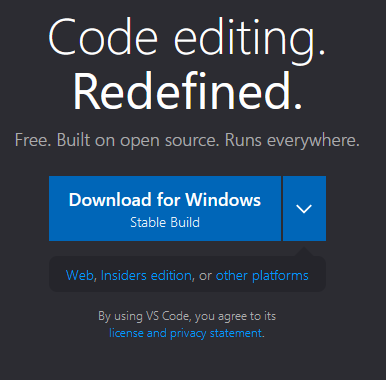
\includegraphics[scale=0.5]{vsc-download}
    \caption{Stranica za preuzimanje VSC-a.}\label{fig:figure8}
\end{figure}

Nakon toga pritisnite \("\)Download for Windows\("\).
Započeti će preuzimanje instalatora za VSC\@.
Kada otvorite instalator, prihvatite licenciju za korištenje, koju ste naravno pročitali od početka do kraja.
Ako želite možete promjeniti mjesto gdje će se VSC instalirati, ali to vjerojatno nije potrebno.
Nakon toga samo završite instalaciju bez dodatnih promjena.

\subsubsection{Korištenje}

Kada otvorite VSCode, dočekati će vas više-manje prazan prozor s nekoliko opcija.
Da bi otvorili projekt, prvo napravite mapu gdje želite da vam se projekt nalazi.
Nakon toga u izborniku na vrhu pritisnite opcju \verb|File| i onda \verb|Open Folder| te izaberite mapu u kojoj želite da se vaš projekt nalazi.

Ta će se mapa otvoriti.
Pod izbornikom \verb|File| možete napraviti novu datoteku, ali isto možete i brže napraviti pomoću izbornika na Slici 1.5.
\begin{figure}[h]
    \centering
    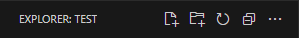
\includegraphics[scale=1]{quick-file-creation-vsc}
    \caption{Brza izrada novih datoteka i mapa u VSC-u.}\label{fig:figure2}
\end{figure}

VSCode, kao i svaki drugi IDE, ima integrirani terminal.
Terminal je tekstualno sučenje za pristup računalu.
Često je brže odraditi nešto pomoću terminala nego pomoću grafičkog sučelja.
Pokreće se pomoću izbornika \verb|Terminal| na vrhu i pritiskom na tipku \verb|New Terminal|.

VSCode podržava inteligentnu podršku tijekom programiranja.
U slučaju VSC-a, a ponekad i drugih IDE-ova, to se zove \textbf{IntelliSense}.

\mlenma{Kako radi IntelliSense}{
    IntelliSense, inteligentno razumjevanje koda, zapravo nije zasluga samog VSCode-a.
    Alatni paketi gotovo svih jezika dolaze s jezičnim poslužiteljem (engl. \textit{language server}).
    To je program koji je zaslužan za analiziranje koda i izdavanje preporuka programeru.
    Te su preporuke onda prenesene IDE-u pomoću protokola jezičnog poslužitelja (engl. \textit{language server protocol}, \textbf{LSP}).
    LSP je protokol koji regulira komunikaciju između IDE-a i jezičnog poslužitelja pa tako omogućuje da jedan jezični poslužitelj radi za sve IDE-ove koji podržavaju LSP.
    Microsoft je originalno razvio LSP isključivo za VSCode, ali je danas otvoreni standard koji se korsiti i u drugima IDE-ovima.
}

\subsubsection{Ekstenzije}

Jedna od najčešćih svrha za VSCode je upravo web programiranje pa zato VSCode dolazi s ugrađenom podršku za JavaScript, HTML i CSS\@.
To znači da nije nužno instalirati dodatne ekstenzije.
Međutim, one vam mogu olakšati život i dodati podršku za nepodržane alate i programske jezike.

\begin{figure}[h]
    \centering
    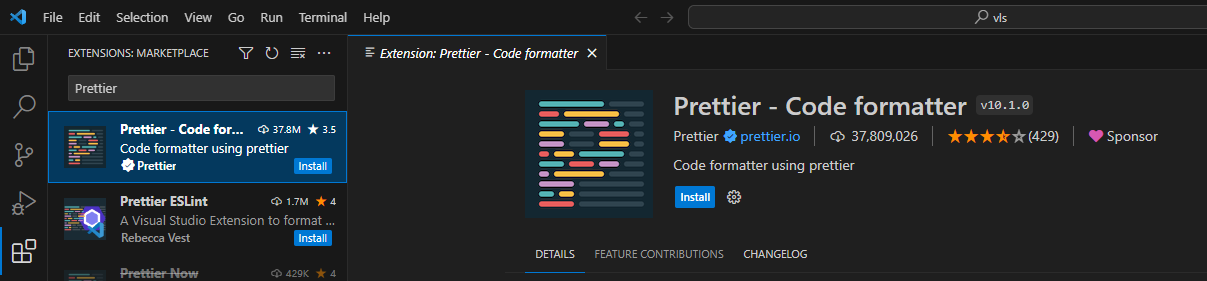
\includegraphics[scale=0.4]{vsc-plugin-download}
    \caption{Instalacija VSCode ekstenzija.}\label{fig:figure}
\end{figure}

Prettier je ekstenzija koja služi kao \textbf{formater}, program koji osigurava da je vaš kod napisan u određenom stilu koji vi definirate.
LiveServer olakšava web programiranje tako što automatski primjećuje promjene vašeg koda i osvježava preglednik automatski kada se one dogode.

Ekstenzije se instaliraju kako je prikazano Slici 1.4.
Prvo pritisnite zadnju opciju na lijevom panelu.
Onda upišite naziv željene ekstenzije, nakon toga pritisntie \("\)Install\("\) ispod imena ekstenzije.
Neke ekstenzije zahtjevaju da ponovno pokrenete VSCode nakon instalacije.

\subsection{WebStorm}\label{subsec:webstorm}

Kako bi instalirali WebStorm otvorite stranicu \href{https://www.jetbrains.com/}{https://www.jetbrains.com/} u vašem pregledniku pa na izborniku pod \verb|Developer Tools| izaberite \verb|WebStorm|.

\begin{wrapfigure}{r}{0.5\textwidth}
    
\includegraphics[scale=0.3]{webstorm-download}
    \caption{Stranica za preuzimanje WebStorma.}
\end{wrapfigure}
Pritisnite tipku \verb|Download| kao što je prikazano na Slici 1.6.

WebStorm je komercijalni proizvod, što znači da se plaća.
Međutim, učenici osnovnih i srednjih škola mogu dobiti pristup WebStormu pomoću svojih CARNET email adresa.
Prvo morate otvoriti JetBrains račun otvaranjem stranice \href{https://account.jetbrains.com/login}{https://account.jetbrains.com/login} i pritisnete opciju \verb|Sign Up| za otvaranje novog računa nakon što upišete svoju CARNET email adresu.
Kada to učinite, primiti ćete email na upisanu adresu.
Kliknite na poveznicu u emailu te popunite obrazac na poveznici.

Nakon toga otvorite poveznicu \href{https://www.jetbrains.com/shop/eform/students}{https://www.jetbrains.com/shop/eform/students}.
Provjerite da je izabrana opcija \verb|University email address|.
Neka vaš \verb|Status| bude \verb|I'm a student|, a \verb|Level of study| neka bude označen kao \verb|Secondary (middle or high school)|.
Odgovor na pitanje ispod nije važan.
Pod polje \verb|Email address| unesite vašu školsku adresu koju ste koristi kada ste napravili vaš JetBrains račun.
Ostatak obrazca popunite kako piše.

Kada ste ga popunili, pritisnite tipku \verb|Apply for free products|.
Primiti ćete još jedan email na kojem će biti još jedan poveznica koju ćete otvoriti.
Jednom kada ste to napravili, i ako ne piše da se dogodila greška, trebali bi imati pristup svim JetBrains proizvodima.

\begin{figure}[h]\label{fig:figure3}
    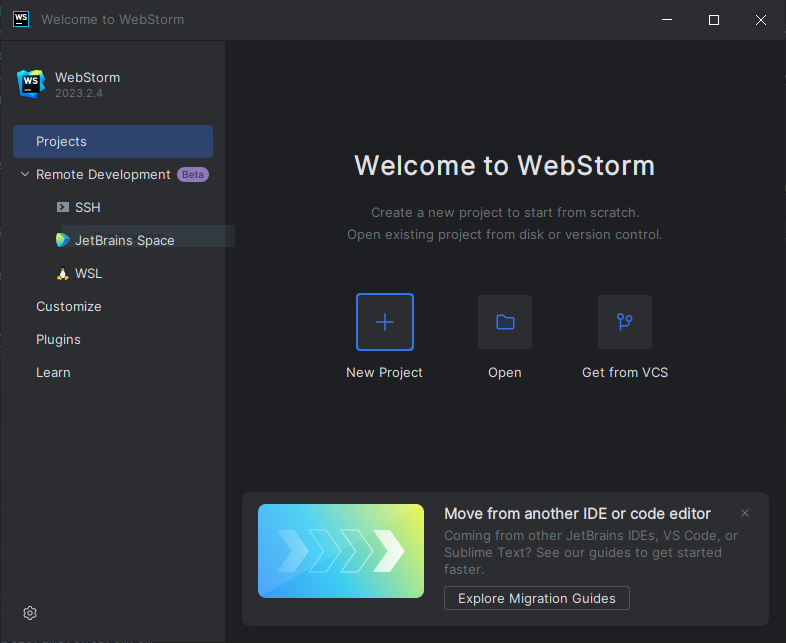
\includegraphics[scale=0.375]{webstorm-home-screen}
    \caption{Početni ekran WebStorma nakon instalacije.}
\end{figure}

Otvorite instalator koji ste ranije preuzeli te samo pratite upute, ne treba mjenjati konfiguraciju instalacije.
Pokrenite WebStorm, trebali bi vidjeti ekran na Slici 1.7.

\subsubsection{Korištenje}

Novi projekt napravite klikom na tipku \verb|New Project|.
Odaberite opciju \verb|Empty Project| na izborniku.
WebStorm dolazi s nekoliko predložaka za projekte s raznim alatima, ali za sada ih nećemo koristiti.
Možete promjeniti gdje će se vaš projekt nalaziti.
To nije nužno, ali možete promjeniti naziv projekta tako što promjeniti naziv mape.
Zadani naziv je \verb |untitled|.
Pritiskom na tipku \verb|Create| stvorit ćete prazan projekt.

Novu datoteku možete stvoriti desnim klikom na željenu lokaciju datoteke ili mape.
WebStorm dolazi sa predložcima za razne vrste (ekstenzije) datoteka.
HTML datoteku možete lako pokrenuti tako što kliknete na zelenu tipku na Slici 1.8.
WebStorm će automatski pratiti promjene koda i osvježavati preglednik.

\begin{figure}[h]
    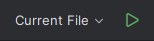
\includegraphics[scale=1]{webstorm-run-file}
    \caption{Pokretanje datoteke u WebStormu.}\label{fig:figure5}
\end{figure}

\subsubsection{Ekstenzije}

\begin{figure}[h]
    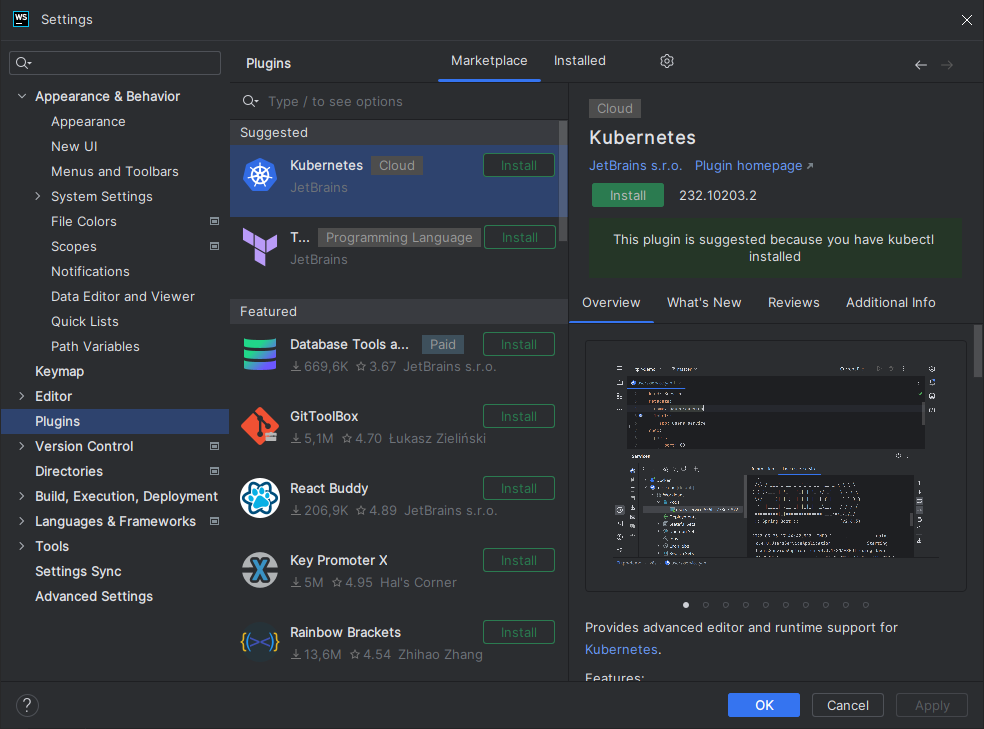
\includegraphics[scale=0.5]{webstorm-plugin-download}
    \caption{Preuzimanje plugina u WebStormu.}\label{fig:figure4}
\end{figure}

Kao i VSCode, WebStorm podržava ekstenzije.
WebStorm dolazi sa gotovo svim potrebnim alatima za web programiranje pa nema tolike potrebe za instaliranjem ekstenzija.
Ekstenzije (ili \textit{Plugini}) se instaliraju pomoću izbornika \verb|Settings| koje se nalaze pod izbornikom \verb|File| u gornjem lijevom kutu.
Pripazite da je izabran \verb|Marketplace|, a ne \verb|Installed|.
Upišite ime plugina i onda pritsnite \verb|Install|.
Možda ćete morati resetirati WebStorm nakon instalacije određenih plugina.

\subsection{Konvencije za imena}\label{subsec:konvencije-za-imenovanje-struktura}

Imena mapa, datoteka i ostalih struktura korištenih za progrmairanje (funkcije, varijable, klase, enumeracije, itd.) u pravilu nemaju razmake, posebne znakove (uključujući i č, ć, ž) i obično su na engleskom.
Postoje četiri naječešće konvencije za imenovanje mapa, datoteka, varijabla, funkcija, itd.
Glavna razlika između njih je način na koji pretstavljaju razmake.

Prva je \textit{\textbf{camelCase}}.
Tako bi recimo naziv \verb|Create Instagram post| bio napisan kao \verb|createInstagramPost|.
Prva riječ započinje s malim slovom, a sve ostale s velikim slovom.
CamelCase jedna je od najkorištenijih konvencija.
U jezicima kao što su Java, JavaScript, Kotlin i Go se koristi za imena struktura u jeziku, funkcije, varijable i sličon.

Druga je \textit{\textbf{PascalCase}}.
Jedina razlike između PascalCase-a i camelCase-a je ta da se u PascalCase-u sve riječi pišu velikim slovima.
\verb|Create Instagram post| bio bi zapisan kao \verb|CreateInstagramPost|
U većini jezika se koristi za nazive kompleksnih tipova podataka (klasa, enumeracija, itd.) te u nekim JavaScript alatima.
U C\#-u se koristi za većinu naziva.

Treća je \textit{\textbf{snake\_case}}.
Sve se riječi pišu malim slovom, a razmaci su zamjenjeni s donjom crticom, \verb|_|.
\verb|Create Instagram post| bio bi zapisan kao \verb|create_instagram_post|.
Koristi se u Pythonu i Rustu za većinu imena, a u Go-u za nazive datoteka.

Zadnja konvencija je \textit{\textbf{kebab-case}}.
Slična je kao \verb|snake_case|, ali umjesto donje crtice se koristi gornja critca, \verb|-|.
\verb|Create Instagram post| bio bi zapisan kao \verb|create-instagram-post|.

\newpage
\section{Uvod u HTML}\label{sec:uvod-u-html}

\textbf{HTML} je programski jezik koji se koristi za definiranje strukture web stranice.
Struktura web stranice je način na koji se određeni dijelovi stranice odnose na druge.
Pomoću HTML-a se ne odreduje izgled stranice ili kako radi.
HTML je napravio Tim Berners-Lee 1991.\ kada je napravio World Wide Web.
Berners-Lee je bio inspiriran jednim sličnim jezikom, \textbf{SGML} (engl. \textit{Standard Generalized Markup Language}).

HTML se zapisuje u \verb|.html| datotekama.\footnote{\texttt{.html} se odnosi na \textbf{ekstenziju} (ili nastavak) datoteke. Ekstenzije govore operacijskom sustavu svrhu datoteke.}
\verb|.html| datoteke su zapravo obične tekstualne datoteke.
Preporučujem vam da upalite vidljivost ekstenzija datoteka na vašem operacijskom sustavu ako već niste.

Napravite novu HTML datoteku.
Ime datoteke nije bitno, ali je bitno da je nastavak \verb|.html|, npr. \verb|uvod-u-html-1.html|.

\lstinputlisting[language=HTML, label={lst:lstinputlisting}, caption={Osnovna struktura HTML dokumenta.}]{kod/p1/uvod-u-html-1.html}

Ako ste sve uspješno napravili, trebali bi pomoći otvoriti tu datoteku u vašem pregledniku klikom na nju i vidjeti da piše \verb|Hello, world!| na stranici.

\subsection{\texttt{<!doctype html>}}\label{subsec:doctype-html}

Svaka HTML datoteka započinje s ovom linjom koda, \verb|<!doctype html>|.
Alternativni zapis je \verb|<!DOCTYPE html>|.
Oba dva zapisa su jedanka.
Ta linija koda govori pregledniku da se radi o HTML dokumentu.

\subsection{\texttt{<html lang="en">}}\label{subsec:html}

Sljedeći dio HTML datoteke je \lstinline!<html>! \textbf{tag}.
HTML tagovi se zapisuju u obliku \lstinline!<tag></tag>!.
Tagovi su osnovni dio HTML-a na osnovnu kojih radi cijeli HTML.
Većina tagova ima otvarajući tag, \lstinline!<tag>! i zatvarajući tag, \lstinline!</tag>!.
Međutim, neki tagovi su samozatvarajući.
Kasnije ćemo pregledati primjere takvih tagova.

Svaki HTML dokument ima jedan element najviše razine, taj element je uvijek \lstinline!<html></html>!.
Unutar njega se nalaze svi drugi elementi.
Kao što vidite, unutar otvarajućeg taga \lstinline!html! elementa nalazi se \lstinline!lang="en"! \textbf{atribut}.
HTML atributi koriste se za prilagođavanje funkcije elementa.
Oblik atributa je uvijek \lstinline!ime="vrijednost"! i uvijek se nalaze unutar otvarajućeg taga elementa, nikad zatvarjućeg.
Dakle, oblik \lstinline!<html></html lang="en">! nije točan.
U ovom slučaju, \lstinline!lang! atribut govori web pregledniku na kojem jezik je tekst web stranice napisan.
Svaki jezik ima svoji pripadajući kod, za engleski je to \lstinline!en!, za hrvatski \lstinline!hr!, njemački \lstinline!de!, itd.
Jezične kodove definira standard ISO 639--1, cijeli popis možete pronaći na \href{https://bit.ly/iso-639-1-kodovi}{https://bit.ly/iso-639-1-kodovi}.

\subsection{\texttt{<head></head>}}\label{subsec:head}

Uz sam \lstinline!<html>! tag, prvi dio HTML datoteke je \lstinline!<head>! element.
\lstinline!<head>! element je obično relativno kratak jer sadrži osnovne podatke o samoj web stranici, naslov, ikonu, i slične podatke.
U ovom slučaju, jedina dva elementa unutar \lstinline!head! taga su elementi \lstinline!<title>Moja web stranica</title>! i \lstinline!<meta charset="UTF-8">!.

\lstinline!<title>! tag je vrlo jednostavan, određuje naslov stranice, tekst koji će biti prikazan u kartici na pregledniku.
\begin{figure}[h]
    
\includegraphics[scale=1]{web-page-title}
    \caption{Naslov web stranice u kartici web preglednika definiran \lstinline!<title>! tagom.}
\end{figure}

\lstinline!<title>! tag, niti bilo što unutar \lstinline!<head>! elementa, neće izravno promjeniti sam sadržaj stranice.
To je dužnost \lstinline!<body>! taga.

Sljedeći tag unutar \lstinline!<html>! taga je \lstinline!<meta charset="UTF-8">!.
Ovaj tag je malo kompliciraniji od \lstinline!<title>! taga.
Za početak, primjetite da je ovaj tag \textbf{samozatvarajući}: tag koji otvara element isto ga i zatvara, odnosno element nema zatvarajući tag.
Nadalje, \lstinline!<meta>! tag ima i druge funkcije, ali ovdje dolazi s \lstinline!charset="UTF-8"! atributom.
Ovdje je \lstinline!charset! kratica za \textit{character set} (skup znakova).
\textbf{UTF-8} jedan je takav skup znakova.\footnote{UTF-8 tehnički nije skup znakova nego način zapisivanja (enkodiranja) Unicode standarda, koji sadrži gotovo sve jezične znakove na svijetu.}
UTF-8 omogućuje zapisivanje gotovo svih postojećih jezičnih znakova na svijetu.

Postoje i drugi \textit{charseti}, ali UTF-8 je najbolji zbog već navedenog razloga.
Jedan poznati primjer je \textbf{ASCII} koji sadrži samo osnovnih 128 engleskih znakova.

\subsection{\texttt{<body></body>}}\label{subsec:body}

\lstinline!<body>! tag je glavni dio HTML datoteke.
On definira sadržaj stranice.

\begin{figure}[h]
    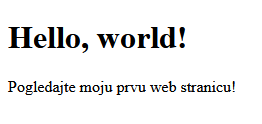
\includegraphics[scale=0.8]{intro-html-1-page-body}
    \caption{Sadržaj web stranice stvoren od koda u Popisu 1.1.}
\end{figure}

\lstinline!<body>! tag može sadržavati bilo kakav tekst.
Ako taj tekst nije unutar nekog taga biti će prikazan kao običan tekst bez ikakvog formatiranja.
Međutim, ovdje je tekst unutar dva taga, \lstinline!<h1>! i \lstinline!<p>!.
\lstinline!<h1>! je \textit{heading} (naslovni) element, on definira najbitniji tekst na stranici, u većini slučajeva naslov stranice.
\lstinline!<h1>! je naslovni element najvećeg prioriteta, još postoje \lstinline!<h2>!, \lstinline!<h3>!, itd.
Web preglednik će automatski tekstu, jer je unutar \lstinline!<h1>! elementa, dodati određene stilove, veliki font i slično.
Tražilice kao što su Google, Bing, Yahoo i ostale će pridati veliku pažnju tekst unutar \lstinline!<h1>! elementa.

Sljedeći element je \lstinline!<p>! \textit{paragraf} element.
\lstinline!<p>! element se koristi za odlomke, odnosno za tekst koji ima prosječnu važnost i, naravno, za velike količine teksta.
Tekst unutar \lstinline!<p>! elementa neće biti od strane web preglednika ili tražilica posebno naglašen.

    %! Author = Karlo
%! Date = 11.11.2023.

% Preamble
\documentclass[11pt]{article}

% Packages
\usepackage{amsmath}

% Document
\begin{document}



\end{document}

\end{document}